\documentclass[12pt]{article}

\usepackage[a4paper,width=160mm,top=20mm,bottom=20mm,bindingoffset=6mm]{geometry}
\usepackage[utf8]{inputenc}
\usepackage[italian]{babel}
\usepackage[OT1]{fontenc}
\usepackage{graphicx}
\usepackage{float}
\usepackage{fancyhdr}
\usepackage{xcolor}
\usepackage{mathtools}
\usepackage{amsmath}
\usepackage{amssymb}
\usepackage{tikz}
\usepackage{imakeidx}
\usepackage{textcomp}
\usepackage{pifont}
\usepackage{polynom}
\usepackage{algorithm}
\usepackage{algpseudocode}
\usepackage{mathtools}
\usepackage[colorlinks=true,linkcolor=black,anchorcolor=black,citecolor=black,filecolor=black,menucolor=black,runcolor=black,urlcolor=black]{hyperref}
\usepackage{cancel}
\usepackage{pgfplots}
\usepackage{caption}
\usepackage{tabularx}
\usepackage{comment}
\usepackage{float}
\usepackage{bm}



\begin{document}
\bibliographystyle{plain}
    \pagestyle{fancy}
    \everymath{\displaystyle}
    \sffamily
    \begin{figure}
        \centering
        
\includegraphics[scale=0.1]{uniba-logo.png}
        \caption*{Università degli Studi di Bari Aldo Moro}
    \end{figure}
    
    \title{Dataset LFM-1b\_artist}
    \author{Emanuele Fontana}
    \date{Tirocinio tesi triennale in Informatica\\Anno accademico 2023/2024}
    \maketitle

    \tableofcontents\newpage

    
\noindent LFM1b\_artist è un dataset contenente informazioni riguardanti le interazioni tra utenti e artisti musicali.

\section*{DETASET ORIGINALE}

\subsection*{STATISTICHE DATASET}


Descrizione del dataset
\begin{table}[H]
    \centering
    \footnotesize
    \begin{tabularx}{\textwidth}{|c|X|}
        \hline
        \textbf{Feature} & \textbf{Descrizione} \\
        \hline
        n\_users & 120322 \\
        \hline
        n\_items & 3123496 \\
        \hline
        n\_inter & 65133026 \\
        \hline
        sparsity & 0.9998266933373666 \\
        \hline
    \end{tabularx}
    \caption{Informazioni sul dataset LFM1b\_artist}
    \label{tab:dataset_info}
\end{table}


\noindent Descrizione del knowledge graph
\begin{table}[H]
    \centering
    \footnotesize
    \begin{tabularx}{\textwidth}{|c|X|}
        \hline
        n\_ent\_head & 823213 \\
        \hline
        n\_ent\_tail & 353607 \\
        \hline
        n\_rel & 8 \\
        \hline
        n\_triple & 2114049 \\
        \hline
    \end{tabularx}
    \caption{Informazioni sul knowledge graph del dataset LFM1b\_artist}
    \label{tab:dataset_info}
\end{table}

\newpage
\noindent I nomi delle relazioni presenti nel knowledge graph sono i seguenti:
\begin{itemize}
    \item music.recording.artist
    \item music.recording.releases
    \item music.recording.producer
    \item music.recording.engineer
    \item music.recording.featured\_artists
    \item music.featured\_artist.recordings
    \item music.release.artist
    \item music.artist.release
\end{itemize}

\section*{DATASET PROCESSATO}

\subsection*{DESCRIZIONE}

\noindent Il dataset originale risultava essere troppo grande per le risorse a nostra disposizione, dunque è stato opportunamente processato. In paritcolare sono state svolte le seguenti operazioni
\begin{itemize}
    \item \textbf{Filtraggio:} il dataset è stato filtrato eliminando tutte le interazioni in cui erano coinvolti utenti e/o item con meno di 5 interazioni
    \item \textbf{Sampling:} dopo la fase di filtraggio, è stato effettuato un sampling casuale il cui scopo era quello di ridurre il numero di interazioni. In particolare sono stati selezionati casualmente 20000 utenti e 50000 item e sono state mantenute solo le interazioni in cui erano coinvolti utenti e gli item selezionati
\end{itemize}

\subsection*{STATISTICHE DATASET}


Descrizione del dataset
\begin{table}[H]
    \centering
    \footnotesize
    \begin{tabularx}{\textwidth}{|c|X|}
        \hline
        \textbf{Feature} & \textbf{Descrizione} \\
        \hline
        n\_users & 19481 \\
        \hline
        n\_items & 42547 \\
        \hline
        n\_inter & 900212 \\
        \hline
        sparsity & 0.0.9989313587429705 \\
        \hline
    \end{tabularx}
    \caption{Informazioni sul dataset LFM1b\_artist processato}
    \label{tab:dataset_info}
\end{table}


\noindent Descrizione del knowledge graph
\begin{table}[H]
    \centering
    \footnotesize
    \begin{tabularx}{\textwidth}{|c|X|}
        \hline
        n\_ent\_head & 15509 \\
        \hline
        n\_ent\_tail & 35156 \\
        \hline
        n\_rel & 5 \\
        \hline
        n\_triple & 46827 \\
        \hline
    \end{tabularx}
    \caption{Informazioni sul knowledge graph del dataset LFM1b\_artist processato}
    \label{tab:dataset_info}
\end{table}

\noindent I nomi delle relazioni presenti nel knowledge graph sono i seguenti:
\begin{itemize}
    \item music.recording.artist
    \item music.recording.releases
    \item music.recording.producer
    \item music.recording.engineer
    \item music.recording.featured\_artists
\end{itemize}


\newpage

\section*{ESECUZIONE DEI MODELLI E RISULTATI}

I modelli di recommendation sono stati eseguiti utilizzando questi parametri:
\begin{itemize}
    \item \textbf{Numero di epoche:} 1
    \item \textbf{Train batch size:} 4096
    \item \textbf{Eval batch size:} 1024
    \item \textbf{Numero neighbors per l'ItemKNN:} 20
\end{itemize}


Qui di seguito sono riportati i risultati ottenuti dai modelli di recommendation.
\begin{table}[H]
    \centering
    \footnotesize
    \begin{tabularx}{\textwidth}{|c|c|X|}
        \hline
        \textbf{Nome modello} & \textbf{Esito} & \textbf{Motivo fallimento} \\
        \hline
        ItemKNN & Successo &  \\
        \hline
        Pop & Successo &  \\
        \hline
        Random & Fallito &  Expected all tensors to be on the same device, but found at least two devices, cuda:0 and cpu! (when checking argument for argument tensors in method wrapper\_CUDA\_cat) \\
        \hline
        Simplex & Successo &  \\
        \hline
        ADMMSLIM & Fallito & Terminato in modo anomalo \\
        \hline
        BPR & Successo &  \\
        \hline
        DMF & Successo &  \\
        \hline
        ENMF & Successo &  \\
        \hline
        FISM & Successo &  \\
        \hline
        NCEPLRec & Successo &  \\
        \hline
        SLIMElasticNet & Fallito &  Expected all tensors to be on the same device, but found at least two devices, cuda:0 and cpu! (when checking argument for argument tensors in method wrapper\_CUDA\_cat) \\
        \hline
        CDAE & Successo &  \\
        \hline
        COnvNCF & Successo &  \\
        \hline
        DiffRec & Successo &  \\
        \hline
        EASE & Fallito & Terminato in modo anomalo \\
        \hline
        GCMC & Successo &  \\
        \hline
        LDiffRec & Successo &  \\
        \hline
        MacridVAE & Fallito &  CUDA out of memory. Tried to allocate 664.00 MiB \\
        \hline
        MultiDAE & Successo &  \\
        \hline
        MultiVAE & Successo &  \\
        \hline
        NAIS & Fallito & CUDA out of memory. Tried to allocate 3.97 GiB \\
        \hline
        NeuMF & Successo &  \\
        \hline
        NGCF & Successo &  \\
        \hline
        NNCF & Successo &  \\
        \hline
        LightGCN & Successo &  \\
        \hline
        RecVAE & Rimandato & Tempo di esecuzione non accettabile \\
        \hline
        DGCF & Successo &  \\
        \hline
        LINE & Successo &  \\
        \hline
        NCL & Fallito & No module faiss \\
        \hline
        SGL & Successo & \\
        \hline
        SpectralCF & Successo &  \\
        \hline
        CKE & Successo &  \\
        \hline
        CFKG & Successo &  \\
        \hline
        KGIN & Fallito & mismatch di versione tra PyTorch e torch\-scatter \\
        \hline
        KGNNLS & Successo &  \\
        \hline
        KTUP & Successo &  \\
        \hline
        MKR & Successo &  \\
        \hline
        RippleNet & Successo &  \\
        \hline
    \end{tabularx}
    \caption{Esiti di esecuzione dei modelli}
    \label{tab:dataset_info}
\end{table}



    \newpage
    \subsection{Configurazione}

\subsubsection{Parametri di running}
Qui di seguito vengono riportati i parametri di running dei vari esperimenti effettuati.


\noindent \textbf{Parametri di environment}


\noindent I parametri di environment servono per configurare l'ambiente di esecuzione.
\begin{itemize}
    \item \textbf{gpu\_id}: 0
    \item \textbf{worker}: 0
    \item \textbf{use\_gpu}: True
    \item \textbf{seed}: 2020
    \item \textbf{state}: INFO
    \item \textbf{encoding}: utf-8
    \item \textbf{reproducibility}: True
    \item \textbf{shuffle}: True
\end{itemize}


\noindent \textbf{Parametri di training}


\noindent I parametri di training servono per l'addestramento dei modelli.
\begin{itemize}
    \item \textbf{epochs}: 200
    \item \textbf{train\_batch\_size}: 2048
    \item \textbf{learner}: adam
    \item \textbf{learning\_rate}: .001
    \item \textbf{train\_neg\_sample\_args}: 
    \begin{itemize}
        \item \textbf{distribution}: uniform
        \item \textbf{sample\_num}: 1
        \item \textbf{dynamic}: False
        \item \textbf{candidate\_num}: 0
    \end{itemize}
    \item \textbf{eval\_step}: 1
    \item \textbf{stopping\_step}: 10
    \item \textbf{clip\_grad\_norm}: None
    \item \textbf{loss\_decimal\_place}: 4
    \item \textbf{weight\_decay}: .0
    \item \textbf{require\_pow}: False
    \item \textbf{enable\_amp}: False
    \item \textbf{enable\_scaler}: False
\end{itemize}


\noindent \textbf{Parametri di evaluation}


\noindent I parametri di evaluation servono per valutare i modelli.
\begin{itemize}
    \item \textbf{eval\_args}:
    \item \begin{itemize}
                \item \textbf{group\_by}: user
                \item \textbf{order}: RO
                \item \textbf{split}: RS : [0.8, 0.1, 0.1]
                \item \textbf{mode}: full
            \end{itemize}
    \item \textbf{repeatable}: False
    \item \textbf{metrics}: ['Recall', 'MRR', 'NDCG', 'Hit', 'MAP', 'Precision', 'GAUC', 'ItemCoverage', 'AveragePopularity', 'GiniIndex', 'ShannonEntropy', 'TailPercentage']
    \item \textbf{topk}: 10
    \item \textbf{valid\_metric}: MRR@10
    \item \textbf{eval\_batch\_size}: 4096
    \item \textbf{metric\_decimal\_place}: 4
\end{itemize}


\noindent \textbf{Iper parametri dei modelli}


\noindent Gli iper parametri dei modelli sono un insieme di parametri che vengono utilizzati per configurare i modelli. La loro configurazione può influenzare il risultato finale. Esistono delle tecniche di HyperTuning che permettono di trovare i migliori iper parametri per un determinato modello e dataset.
In questo caso si è scelto di utilizzare gli iper parametri di default



    \newpage
    \section{Emissioni}

Qui di seguito vengono riportate le emissioni di CO2 per ogni esperimento effettuato.

\begin{table}[H]
    \centering
    \footnotesize
    \setlength\tabcolsep{0pt}
    \begin{tabularx}{\textwidth}{|X|X|}
        \hline
        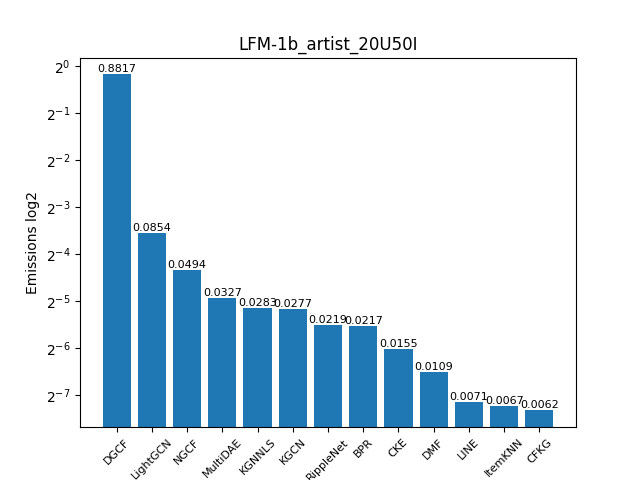
\includegraphics[width=\linewidth, trim=0 0 0 0]{images/emissions_LFM-1b_artist_20U50I.png} &
        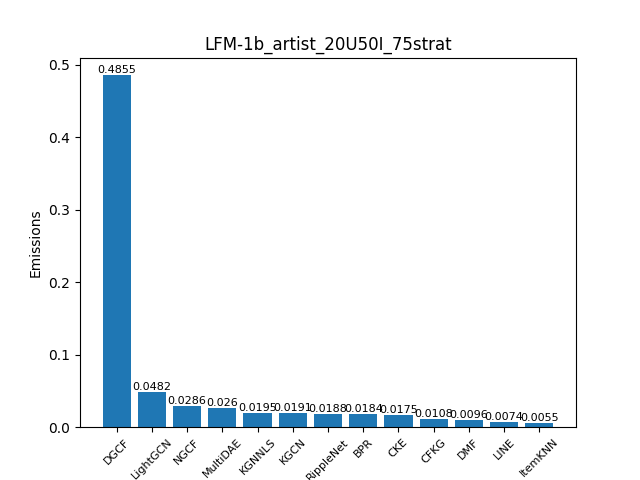
\includegraphics[width=\linewidth, trim=0 0 0 0]{images/emissions_LFM-1b_artist_20U50I_75strat.png} \\
        \hline
        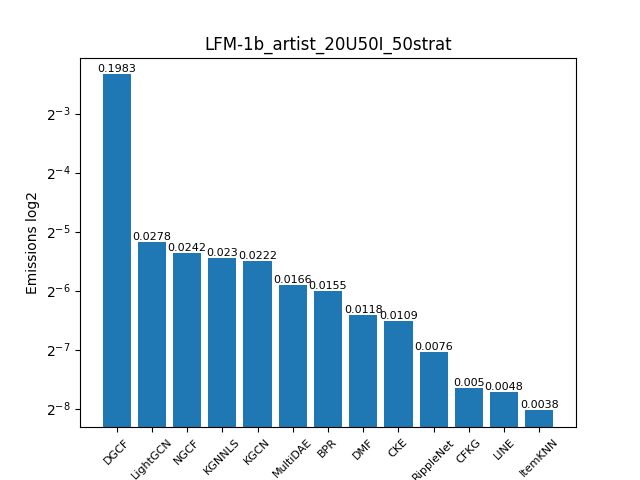
\includegraphics[width=\linewidth, trim=0 0 0 0]{images/emissions_LFM-1b_artist_20U50I_50strat.png} &
        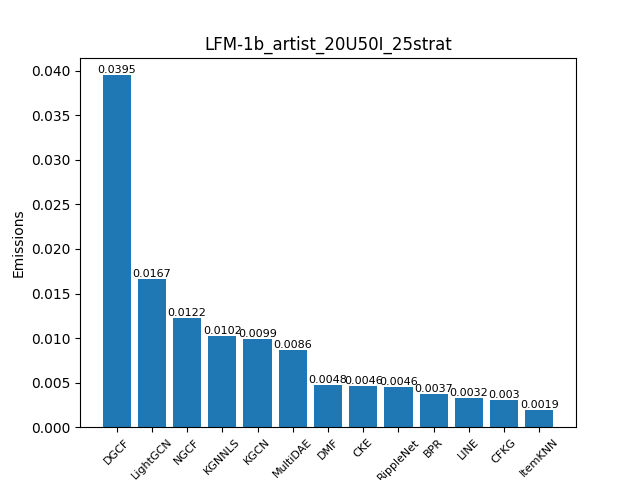
\includegraphics[width=\linewidth, trim=0 0 0 0]{images/emissions_LFM-1b_artist_20U50I_25strat.png} \\
        \hline
    \end{tabularx}
    \caption{Emissioni di CO2 per i vari dataset}
    \label{tab:emissions_info}
\end{table}

\noindent Si può subito notare come DGCF è il modello che emette più CO2 in assoluto.
In particolare con il dataset al 100\% e al 75\% DGCF emette circa 10 volte di più rispetto a LightGCN (il secondo per emissioni)
mentre con il dataset al 50\% emette circa 7 volte di più e con il dataset al 25\% emette circa 2 volte di più (sempre rispetto a LightGCN).
LightGCN e NCFG sono rispettivamente il secondo e il terzo modello che emettono più CO2.
Questi due modelli sono invece di tipo general, ma nonostante ciò emettono di più rispetto ad altri di tipo knowledge-aware, come per esempio il KGCN.
In generale possiamo vedere che ItemKNN,LINE e CFKG sono i modelli che emettono meno.
Per LINE e ItemKNN questo era abbastanza prevedibile in quanto modelli di tipo General. Interessante invece notare come CFKG, di tipo knowledge-aware, emetta meno di altri modelli di tipo General






    \newpage
    \subsection{Trade-off}


\subsubsection{Introduzione}
In questa sezione verranno analizzati i trade-off tra le varie metriche di valutazione e le emissioni di CO2 analizzando un dataset per volta.

Di seguito un elenco delle metriche con una piccola descrizione:
\begin{itemize}
    \item \textbf{Recall}: è una metrica che misura la capacità di un modello di raccomandare gli item rilevanti per un utente
    \item \textbf{NDCG}: è una metrica che misura la qualità delle raccomandazioni.
    \item \textbf{Gini Index}: è una metrica che misura l'equità nella distribuzione delle raccomandazioni. Un valore più vicino a zero indica una distribuzione più equa
    \item \textbf{Average Popularity}: è una metrica che misura la popolarità media degli item raccomandati. Un valore alto indica che le raccomandazioni sono concentrate su item popolari.
\end{itemize}

\subsubsection{LFM-1b\_artist\_20U50I}


\begin{table}[H]
    \centering
    \footnotesize
    \setlength\tabcolsep{0pt}
    \begin{tabularx}{\textwidth}{|X|X|}
        \hline
        \includegraphics[width=\linewidth, trim=0 0 0 0]{images/recall@10\_LFM-1b\_artist_20U50I.png} &
        \includegraphics[width=\linewidth, trim=0 0 0 0]{images/ndcg@10\_LFM-1b\_artist_20U50I.png} \\
        \hline
        \includegraphics[width=\linewidth, trim=0 0 0 0]{images/giniindex@10\_LFM-1b\_artist_20U50I.png} &
        \includegraphics[width=\linewidth, trim=0 0 0 0]{images/averagepopularity@10\_LFM-1b\_artist_20U50I.png} \\
        \hline
    \end{tabularx}
    \caption{Trade-off con il dataset LFM-1b\_artist\_20U50I}
    \label{tab:emissions_info}
\end{table}

\noindent Come già visto precedentemente, DGCF è il modello che emette di più. Nonostante ciò possiamo notare che per la recall e l'ndcg le sue performance risultano peggiori rispetto ad algoritmi più semplici come l'ItemKNN che risulta essere uno degli algoritmi che emette meno e performa meglio in queste metriche.
Per quanto riguarda il Gini Index possiamo notare che DGCF si comporta meglio di molti altri modelli ma l'ItemKNN e LINE risultano essere migliori di quest'ultimo. LINE è il miglior algoritmo.
Infine, per quanto riguarda l'Average Popularity, anche in questo caso possiamo notare anche che DGCF performa meglio di altri modelli, ma LINE risulta il miglior in assoluto ed è uno degli algoritmi che emette meno.


\subsubsection{LFM-1b\_artist\_20U50I\_75strat}


\begin{table}[H]
    \centering
    \footnotesize
    \setlength\tabcolsep{0pt}
    \begin{tabularx}{\textwidth}{|X|X|}
        \hline
        \includegraphics[width=\linewidth, trim=0 0 0 0]{images/recall@10\_LFM-1b\_artist_20U50I\_75strat.png} &
        \includegraphics[width=\linewidth, trim=0 0 0 0]{images/ndcg@10\_LFM-1b\_artist_20U50I\_75strat.png} \\
        \hline
        \includegraphics[width=\linewidth, trim=0 0 0 0]{images/giniindex@10\_LFM-1b\_artist_20U50I\_75strat.png} &
        \includegraphics[width=\linewidth, trim=0 0 0 0]{images/averagepopularity@10\_LFM-1b\_artist_20U50I\_75strat.png} \\
        \hline
    \end{tabularx}
    \caption{Trade-off con il dataset LFM-1b\_artist\_20U50I\_75strat}
    \label{tab:emissions_info}
\end{table}


\noindent Come già visto precedentemente, DGCF è il modello che emette di più. Nonostante ciò possiamo notare che per la recall e l'ndcg le sue performance risultano peggiori rispetto ad algoritmi più semplici come l'ItemKNN che risulta essere uno degli algoritmi che emette meno e performa meglio in queste metriche.
Per quanto riguarda il Gini Index possiamo notare che DGCF si comporta meglio di molti altri modelli ma l'ItemKNN e LINE risultano essere migliori di quest'ultimo. ItemKNN è il miglior algoritmo.
Infine, per quanto riguarda l'Average Popularity, anche in questo caso possiamo notare anche che DGCF performa meglio di altri modelli, ma LINE risulta il miglior in assoluto ed è uno degli algoritmi che emette meno.





\subsubsection{LFM-1b\_artist\_20U50I\_50strat}


\begin{table}[H]
    \centering
    \footnotesize
    \setlength\tabcolsep{0pt}
    \begin{tabularx}{\textwidth}{|X|X|}
        \hline
        \includegraphics[width=\linewidth, trim=0 0 0 0]{images/recall@10\_LFM-1b\_artist_20U50I\_50strat.png} &
        \includegraphics[width=\linewidth, trim=0 0 0 0]{images/ndcg@10\_LFM-1b\_artist_20U50I\_50strat.png} \\
        \hline
        \includegraphics[width=\linewidth, trim=0 0 0 0]{images/giniindex@10\_LFM-1b\_artist_20U50I\_50strat.png} &
        \includegraphics[width=\linewidth, trim=0 0 0 0]{images/averagepopularity@10\_LFM-1b\_artist_20U50I\_50strat.png} \\
        \hline
    \end{tabularx}
    \caption{Trade-off con il dataset LFM-1b\_artist\_20U50I\_50strat}
    \label{tab:emissions_info}
\end{table}


\noindent Come già visto precedentemente, DGCF è il modello che emette di più. Nonostante ciò possiamo notare che per la recall e l'ndcg le sue performance risultano peggiori rispetto ad altri algoritmi che emettono meno come CKE e CKFG(anch'essi di tipo Knowledge-Aware)..
Per quanto riguarda il Gini Index possiamo notare che DGCF si comporta meglio di molti altri modelli ma l'ItemKNN risulta essere migliore di quest'ultimo ed il migliore in assoluto.
Infine, per quanto riguarda l'Average Popularity, anche in questo caso possiamo notare anche che DGCF performa meglio di altri modelli, ma LINE risulta il miglior in assoluto ed è uno degli algoritmi che emette meno.



\subsubsection{LFM-1b\_artist\_20U50I\_25strat}


\begin{table}[H]
    \centering
    \footnotesize
    \setlength\tabcolsep{0pt}
    \begin{tabularx}{\textwidth}{|X|X|}
        \hline
        \includegraphics[width=\linewidth, trim=0 0 0 0]{images/recall@10\_LFM-1b\_artist_20U50I\_25strat.png} &
        \includegraphics[width=\linewidth, trim=0 0 0 0]{images/ndcg@10\_LFM-1b\_artist_20U50I\_25strat.png} \\
        \hline
        \includegraphics[width=\linewidth, trim=0 0 0 0]{images/giniindex@10\_LFM-1b\_artist_20U50I\_25strat.png} &
        \includegraphics[width=\linewidth, trim=0 0 0 0]{images/averagepopularity@10\_LFM-1b\_artist_20U50I\_25strat.png} \\
        \hline
    \end{tabularx}
    \caption{Trade-off con il dataset LFM-1b\_artist\_20U50I\_25strat}
    \label{tab:emissions_info}
\end{table}


\noindent Come già visto precedentemente, DGCF è il modello che emette di più. Nonostante ciò possiamo notare che per la recall e l'ndcg le sue performance risultano peggiori rispetto ad altri algoritmi che emettono meno come CKE e CKFG (anch'essi di tipo Knowledge-Aware).
Per quanto riguarda il Gini Index possiamo notare che DGCF si comporta meglio di molti altri modelli ma l'ItemKNN risulta essere di quest'ultimo migliore ed il migliore in assoluto.
Infine, per quanto riguarda l'Average Popularity, in questo caso possiamo notare anche che DGCF è uno dei peggiori mentre ItemKNN risulta il miglior in assoluto ed è l'algoritmo che emette meno.


\subsubsection{ml-10m\_50U10I}


\begin{table}[H]
    \centering
    \footnotesize
    \setlength\tabcolsep{0pt}
    \begin{tabularx}{\textwidth}{|X|X|}
        \hline
        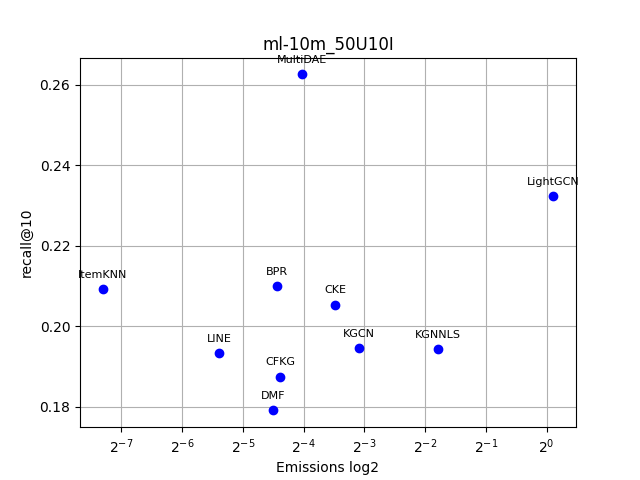
\includegraphics[width=\linewidth, trim=0 0 0 0]{images/recall@10_ml-10m_50U10I.png} &
        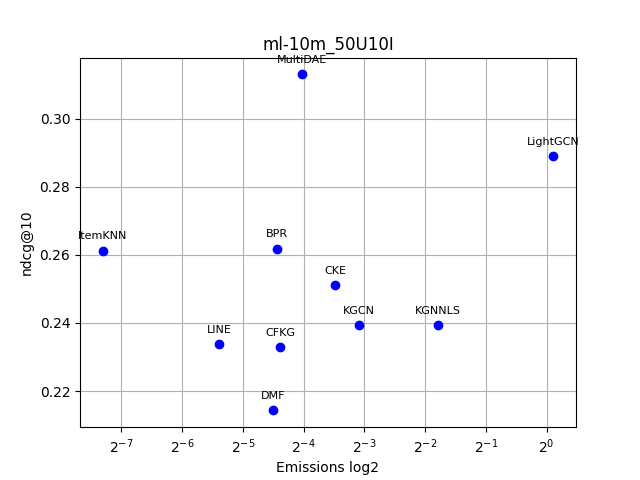
\includegraphics[width=\linewidth, trim=0 0 0 0]{images/ndcg@10_ml-10m_50U10I.png} \\
        \hline
        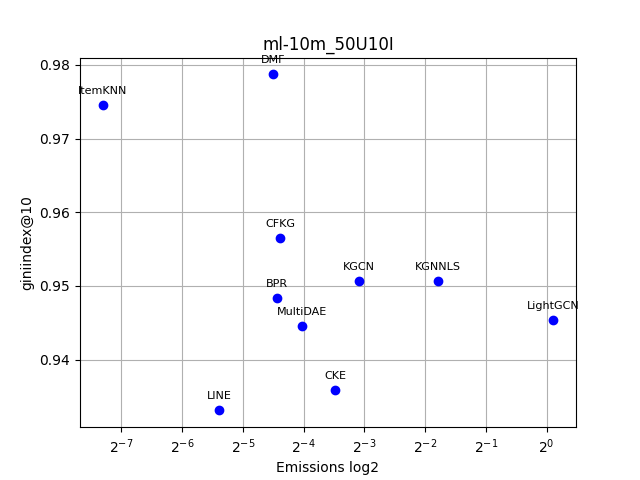
\includegraphics[width=\linewidth, trim=0 0 0 0]{images/giniindex@10_ml-10m_50U10I.png} &
        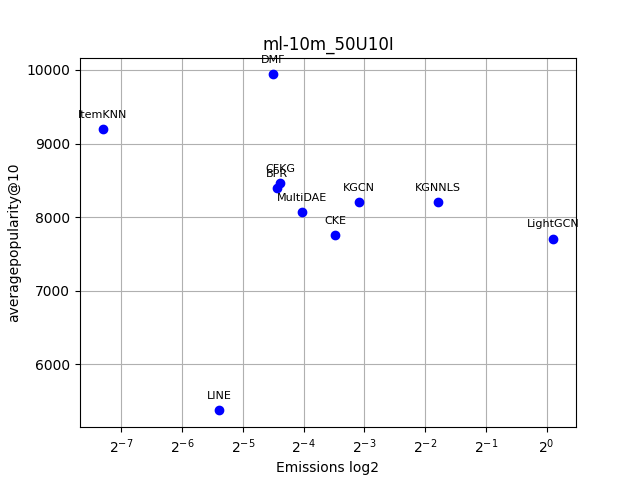
\includegraphics[width=\linewidth, trim=0 0 0 0]{images/averagepopularity@10_ml-10m_50U10I.png} \\
        \hline
    \end{tabularx}
    \caption{Trade-off con il dataset ml-10m\_50U10I}
    \label{tab:emissions_info}
\end{table}

\noindent LightGCN è l'algoritmo che emette di più, osservando i valori da 5 a circa 180 volte rispetto agli altri modelli.
Emissioni cosi alte non sono però giustificate. Nelle metriche di recall e ndcg LightGCN è il secondo migliore, ma la differenza rispetto al primo è molto bassa e quindi non giustifica emissioni così alte.
ItemKNN si conferma uno dei migliori algoritmi per queste due metriche in quanto emette meno ed è uno dei più performanti.
Per quanto riguarda le metriche di Gini Index e Average Popularity possiamo notare che LightGCN è uno di migliori, ma anche in questo caso la differenza rispetto ad altri modelli non giustifica emissioni così alte. ItemKNN si conferma con il secondo peggior modello come punteggi. Line risulta essere il migliore in quanto è il secondo per basse emissioni ed ottiene i punteggi migliori. 

\subsubsection{Conclusioni}

Si può facilmente notare come il trade-off emissioni-performance sia decisamente a svantaggio dell'DGCF. Infatti, a fronte di emissioni molto elevate, le performance risultato spesso essere peggiori di modelli molto più semplici.
Con i due dataset più grandi possiamo notare come in generale ItemKNN risulti essere uno degli algoritmi con il miglior trade-off emissioni-performance nelle metriche di ranking, mentre LINE risulta essere il migliore nelle metriche di popolarità e equità nelle distribuzioni.
Al diminuire della dimensione del dataset DGCF comincia a comportarsi meglio nelle metriche di popolarità e equità, ma le sue emissioni rimangono sempre molto alte e non giustificano una possibile scelta di questo modello.
ItemKNN comincia a non performare bene nelle metriche di ranking, mentre migliora nelle metriche di popolarità e equità, arrivando anche a risultare il migliore


    \newpage
    \section{Conclusioni e sviluppi futuri}
\subsection{Conclusioni}
Vengono qui brevemente riassunti i risultati ottenuti e le conclusioni a cui si è giunti in seguito al lavoro svolto.
\begin{itemize}
    \item \textbf{Benchmarking}: Vengono confermate le ipotesi iniziali per cui modelli più complessi emettono molta più CO2 rispetto a modelli più semplici senza però ottenere un miglioramento significativo delle metriche di valutazione (a volte addirittura peggiori). Si può notare inoltre come alcuni modelli tendono ad avere performance simili con qualsiasi dataset, mentre altri variano molto in base al dataset utilizzato.
    \item \textbf{Lavoro sul regressore}: Il regressore proposto ha ottenuto risultati peggiori rispetto al lavoro iniziale. Il dataset a disposizione sicuramente risulta essere più grande e vario nelle feature di input rispetto a quello utilizzato inizialmente, ma risultata essere molto sbilanciato nella feature di output in quando ci sono modelli che, a prescindere dal dataset, svettano rispetto agli altri in emissioni di molto e ciò ha portato il regressore a non riuscire a generalizzare bene
    \item \textbf{Addestramento sostenibile}: Il lavoro svolto ha portato a risultati interessanti. Si è dimostrato che è possibile addestrare un modello di Recommender System in maniera sostenibile, riducendo le emissioni di CO2 rispetto all'addestramento standard mantenendo però delle performance accettabili. Sono anche stati individuati dei pattern che possono aiutare a comprendere quali parametri del criterio di early stopping influenzino maggiormente l'addestramento in determinati contesti.
\end{itemize}
\subsection{Sviluppi futuri}
Il lavoro svolto ha dunque sicuramente mosso dei passi in avanti in ambito Recommender Systems e sostenibilità ambientale, ma siamo solo agli inizi. Ci sono diverse direzioni in cui si potrebbe andare per migliorare il sistema proposto:
\begin{itemize}
    \item \textbf{Benchmarking}: E' necessario effettuare più esperimenti variando i dataset, i modelli ma sopratutto l'hardware su cui si effettuano gli addestramenti. Questo permetterebbe di avere una visione più chiara delle prestazioni in relazione alle emissioni di CO2.
    \item \textbf{Lavoro sul regressore}: Con molti più dati a disposizione il regressore potrebbe essere addestrato su un dataset più grande e più vario. Inoltre, si potrebbero provare diverse architetture di rete neurale (oltre ai classici regressori), altri regressori e lavorare su diversi iperparametri per cercare di ottenere un modello più accurato.
    \item \textbf{Addestramento sostenibile}: Anche in questo caso variare dataset, modelli, hardware e parametri di early stopping (soglia e epoche consecutive) potrebbe portare a risultati interessanti che potrebbero confermare o smentire le ipotesi fatte in questo lavoro.
    \item \textbf{Lavorare sugli iperparametri}: Gli esperimenti effettuati in questo lavoro sono stati effettuati con i parametri di default. Gli stessi esperimenti (Benchmarking, regressore e addestramento sostenibile) potrebbero essere ripetuti con la ricerca degli iperparametri migliori per ogni modello e confrontare poi con i risultati ottenuti con i parametri di default. In questo modo si potrebbe vedere se le emissioni emesse per la ricerca degli iperparametri sono giustificate dai risultati ottenuti (quindi elevati miglioramenti).
\end{itemize}



\end{document}
